\documentclass[11pt,a4paper]{article}
\usepackage[T1]{fontenc}
\usepackage{lmodern,microtype}
\usepackage[margin=2cm,headheight=14pt]{geometry}
\usepackage{amsmath,amssymb,booktabs,tabularx,array}
\usepackage[dvipsnames]{xcolor}
\usepackage{tikz}
\usetikzlibrary{arrows.meta,positioning}
\usepackage{enumitem,fancyhdr,hyperref}
\definecolor{navy}{HTML}{18354A}
\definecolor{teal}{HTML}{166B70}
\hypersetup{colorlinks=true,urlcolor=teal,linkcolor=navy,citecolor=teal,
  pdftitle={Selecting Reliable LLM Reasoning with Answer-Group Preferences},
  pdfauthor={DASE7506 Mini-Project 2}}
\pagestyle{fancy}\fancyhf{}
\fancyhead[L]{\small\textcolor{navy}{DASE7506 \quad Mini-Project 2}}
\fancyhead[R]{\small 29 October 2026}
\fancyfoot[C]{\small\thepage}
\renewcommand{\headrulewidth}{0.3pt}
\setlength{\parindent}{0pt}
\setlength{\parskip}{5pt}
\setlength{\tabcolsep}{5pt}
\renewcommand{\arraystretch}{1.12}
\setlist[itemize]{leftmargin=*,itemsep=2pt,topsep=3pt}
\newcommand{\code}[1]{\texttt{\small #1}}
\newcommand{\R}{\mathbb{R}}
\newcommand{\softplus}{\operatorname{softplus}}
\newcommand{\pageheading}[1]{\section{#1}}
\raggedbottom

\begin{document}
\begin{center}
{\LARGE\bfseries\color{navy} Selecting Reliable LLM Reasoning}\\[4pt]
{\Large with Answer-Group Preferences}\\[7pt]
{\small A compact CPU selector for four fixed mathematical solutions}
\end{center}
\vspace{2pt}
\textbf{Abstract.}
This project studies answer selection rather than solution generation. Given
four supplied traces and fixed embeddings, the selector must choose a candidate
whose final numeric answer is correct. The final method pools numerically
equivalent answers, combines their 1024-dimensional mean embeddings with nine
group/answer descriptors, and fits a linear Bradley--Terry preference model.
Matched training comparisons show that pooling alone hurts: it answers
1596/2114 out-of-fold questions correctly, versus 1682 for candidate-level
preferences. Adding the descriptor block raises this to 1713, with 299/355 on
informative validation questions. The frozen checkpoint obtains
\textbf{387/467 (82.8694\%)} on the official test bank and contains only
\textbf{26,189 bytes} of inference assets. Feature ablations and nested
evaluation of fallback rules support a conservative final design. In particular,
a threshold rule apparently gaining 15 questions when selected on all OOF
predictions loses two under nested evaluation. The principal findings concern
representation, fair comparisons and evaluation reliability, rather than model
size or a claim of verified mathematical reasoning.

\pageheading{Question and scope}
The supplied solutions can be fluent, internally consistent, and still answer
the wrong question. The course benchmark grades the selected \emph{final number},
including equivalent fractions and decimals; it does not grade every reasoning
step. We therefore distinguish selecting a correct answer from certifying a
correct derivation. GSM8K provides the underlying word problems~\cite{gsm8k};
the candidate bank and representations are those supplied by the course~\cite{guide}.

The main research question is:
\begin{quote}
Does exact numeric-answer grouping, together with a small block of group and
answer descriptors, improve a fixed linear preference ranker under CPU limits?
Which parts of the apparent improvement survive fair controls?
\end{quote}

\begin{center}
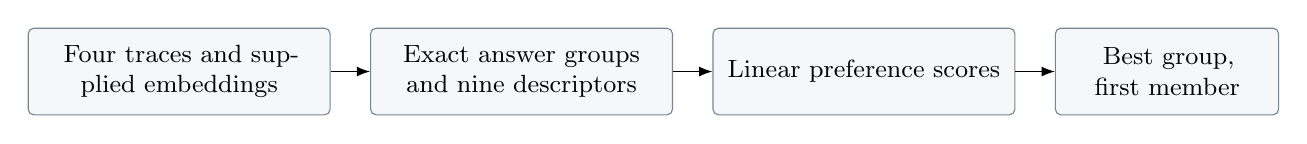
\begin{tikzpicture}[node distance=5mm,box/.style={draw=navy!60,rounded corners=2pt,
  fill=navy!4,align=center,font=\small,minimum height=11mm,text width=36mm},
  >=Latex]
\node[box] (a) {Four traces and\ supplied embeddings};
\node[box,right=of a] (b) {Exact answer groups\ and nine descriptors};
\node[box,right=of b] (c) {Linear preference\ scores};
\node[box,right=of c,text width=26mm] (d) {Best group,\ first member};
\draw[->] (a)--(b);\draw[->] (b)--(c);\draw[->] (c)--(d);
\end{tikzpicture}
\end{center}

The study has three useful outcomes. First, it separates the benefit of the
descriptor block from the unsuccessful pooling-only change. Second, it exposes
how easy validation questions and reuse of OOF predictions can inflate
impressions of reliability. Third, it retains a small, reproducible model after
more elaborate alternatives fail to provide stable evidence of improvement.
No external training data, additional pretrained weights, new solution text or
model API is used by the selector.

\newpage
\pageheading{Data, labels and evaluation protocol}
Each question supplies four candidate texts and a float32 embedding array of
shape $4\times1024$. The official parser maps each final answer to a canonical
rational value, or returns invalid. For training candidate $i$ in question $q$,
the target is
\[
y_{qi}=\mathbf{1}\{a_{qi}\ne\varnothing\ \land\ a_{qi}=a_q^{\mathrm{ref}}\}.
\]
Several candidates may be positive. Labels are aligned by both identifier and
question text; identifiers are never predictive features.

\begin{table}[h]\centering
\caption{The informative subset has at least two distinct valid numeric answers.}
\begin{tabular}{lrrr}\toprule
 & Train & Validation & Test \\\midrule
All supplied questions & 4755 & 798 & 467 \\
Four candidates all correct & 2242 & 379 & -- \\
After removing all-correct questions & 2513 & 419 & -- \\
Informative answer disagreement & 2114 & 355 & 467 \\
Non-all-correct, one valid answer group & 399 & 64 & 0 \\
\bottomrule\end{tabular}
\end{table}

\textbf{Training support.} Final weights and all normalization statistics use
only the 2114 informative training questions. All-correct questions provide no
positive-versus-negative ranking pairs. The further 399 questions contain one
valid answer group and do not teach a preference between valid answers. The
official files are not edited: filtering is an in-memory mask. Earlier MLP
experiments already excluded all-correct questions from their loss, but used
different standardization/support settings; this is a confound in historical
cross-family comparisons.

\textbf{Validation denominators.} We report the complete 798-question bank, the
419 non-all-correct questions when useful, and primarily the 355 informative
questions. Validation contains 443 one-valid-group questions; choosing that group
answers all of them correctly. The final model's 742/798 thus decomposes as
$443+299$. Full validation accuracy is not directly comparable to test, where
all 467 questions require choosing between different valid answers.

\textbf{OOF construction.} Three-fold assignments are generated on all 4755
training rows, before informative filtering. With NumPy \code{default\_rng}
seed 20261028, rows are stratified by disagreement and number of positive
candidates, shuffled within strata and assigned round-robin with a carried
offset. Exact duplicate question texts share the first occurrence's fold. Each
fit and its statistics use informative questions outside its held-out fold.
The informative held-out sizes are 704, 705 and 705. Generating folds only on
the 2114-question subset would change the random sequence and the experiment.

\textbf{Development boundary.} Validation was reused for development and is
not a fresh holdout. Public test references were available for official scoring,
and several frozen historical methods were scored during the project. They did
not enter weight fitting, feature construction or threshold estimation. The
reported test result is therefore a public-bank result, not a claim of a
single-use blinded evaluation. No test error cases are used in this report.

\newpage
\pageheading{Answer groups and compact evidence}
Let $x_{qi}\in\R^{1024}$ denote the supplied candidate embedding. Candidates with
the same valid parsed answer form $G_{qg}$, with answer $a_{qg}$. An unparseable
answer belongs to no valid group. Equivalent forms such as $0.5$ and $1/2$
are pooled exactly, rather than by approximate string or embedding similarity.
The semantic representation of group $g$ is
\[
\bar x_{qg}=\frac{1}{|G_{qg}|}\sum_{i\in G_{qg}}x_{qi}.
\]
This aligns the action space with the scorer: all members of one numeric group
have the same final-answer correctness. However, averaging can discard useful
trace differences. Pooling is consequently a hypothesis to test, not a presumed
improvement over candidate-level scoring.

\begin{table}[h]\centering\small
\caption{Nine descriptors appended to the group mean; no learned text encoder.}
\begin{tabularx}{\linewidth}{@{}lX@{}}\toprule
Descriptor & Definition or implementation \\\midrule
Support fraction & $|G_{qg}|/4$, with the original four slots as denominator. \\
Log variance & $\log(1+v)$, $v=\frac{1}{1024|G|}\sum_{i\in G}\|x_{qi}-\bar x_{qg}\|^2$. \\
Pairwise cosine & Mean cosine over distinct within-group candidate pairs; zero for a singleton. Norms are floored at $10^{-12}$. \\
Signed log magnitude & $\ell(a)=\operatorname{sign}(a)\log(1+|a|)$. \\
Integer flag & Whether the canonical rational answer has denominator one. \\
Zero flag & Whether the answer equals zero. \\
Negative flag & Whether the answer is negative. \\
Exact question number & Whether the answer occurs among rational numeric tokens extracted from the question. \\
Relative magnitude & $\ell(a/M_q)$, where $M_q$ is the largest absolute extracted question number; zero if $M_q=0$. \\
\bottomrule\end{tabularx}
\end{table}

The final feature vector $f_{qg}=[\bar x_{qg};h_{qg}]$ has 1033 dimensions.
Statistics such as group support and variance describe agreement; numeric
descriptors provide low-cost information about the form and scale of an answer.
They are \emph{soft learned evidence}, not hard rules. An integer answer is not
automatically correct, and a minority answer is not automatically wrong.

Question numbers are extracted with a bounded regular expression and exact
rational conversion (at most 20,000 characters and 512 tokens). This does not
interpret units, percentages or the role of a quantity. For example, detecting
an answer already present in a question is different from proving that it is the
requested quantity. These restrictions are both engineering choices and limits
of the evidence available to the model.

The final model contains \emph{no local equation checker} and no explicit
question-mean-centering branch. In the linear embedding component, a common
question-level offset cancels in pairwise differences; the appended cosine
descriptor is not translation-invariant. Earlier nonlinear models
used explicit centering; that earlier design should not be attributed to the
final ranker. Likewise, the nine-dimensional block mixes group statistics and
answer form, so its measured benefit cannot be credited to answer form alone.

\newpage
\pageheading{Preference objective and implementation}
For informative question $q$, there is exactly one correct numeric answer
group $g_q^+$ and $K_q-1$ incorrect valid groups. A linear score is
$s_{qg}=w^\top z_{qg}$, where $z$ is standardized $f$. The Bradley--Terry model
uses $\sigma(s_{qg^+}-s_{qg})$ for a pairwise preference~\cite{bt}. We minimize
\begin{equation}
\mathcal L(w)=\frac{1}{|H|}\sum_{q\in H}\frac{1}{K_q-1}
\sum_{g\ne g_q^+}\log\!\left(1+\exp\{-w^\top(z_{qg_q^+}-z_{qg})\}\right)
+\frac{\lambda}{2}\|w\|_2^2,\qquad \lambda=0.01.
\end{equation}
Each question has total pair weight one; its wrong answer groups share that
weight uniformly. A question with three wrong answers therefore does not count
three times as much as a question with one. Multiple copies of a wrong numeric
answer are collapsed rather than receiving extra negative weight.

For the candidate-level control, all correct/incorrect candidate pairs are
used, but a pair with incorrect group $g$ has weight
$1/[(K_q-1)|G_q^+||G_{qg}|]$. This preserves equal question and wrong-answer-group
mass despite repeated positive or negative candidates. It makes the main
representation comparison more meaningful than an unweighted pair expansion.

\textbf{Train-only normalization.} The 1024 embedding means and scales are
estimated from all four original candidates of informative training questions,
including embeddings of invalid-answer candidates. This convention is shared
by candidate and group controls. The nine appended statistics are normalized
using valid answer groups in the same training support. Standard deviations
are floored at $10^{-6}$. Pooling commutes with the affine embedding transform;
the different descriptor block has its own statistics. Validation and held-out
folds never supply these statistics.

\begin{table}[h]\centering
\caption{The original full-training final fit. Times exclude data loading.}
\begin{tabular}{lr}\toprule
Informative questions / original candidate embeddings & 2114 / 8456 \\
Valid groups / preference pairs & 5172 / 3058 \\
Total pair weight / coefficients & 2114 / 1033 \\
L-BFGS-B iterations / function evaluations & 71 / 80 \\
Maximum absolute final gradient & $5.90\times10^{-7}$ \\
Recorded fit time on the local CPU & 1.0943 s \\
\bottomrule\end{tabular}
\end{table}

Optimization uses deterministic zero initialization, analytic gradients and
SciPy L-BFGS-B: at most 500 iterations, \code{ftol=1e-10}, \code{gtol=1e-7},
and \code{maxls=50}. There is no random training seed, intercept, early stopping
or validation fitting. Numerically stable softplus avoids exponential overflow.

At inference, we select the highest-scoring valid group and return its first
member. Groups and exact ties use first-occurrence order. Thus the selected
\emph{numeric answer} is insensitive to duplicate-member identity, but exact
ties can depend on order. On an all-invalid input, a defined embedding-only
fallback chooses a candidate. The method accepts arbitrary input bank sizes
and reads only passed texts/embeddings and the frozen bundle.

\newpage
\pageheading{Main results and controlled interpretation}
The main comparison holds informative support, folds, normalization convention,
L2 and question/pair weighting fixed. Each representation has three fold fits
and one full fit; validation follows freezing. The difference between the last
two rows is the added descriptor block, not a change of optimizer or support.

\begin{table}[h]\centering
\caption{Matched linear comparisons. OOF and validation have different supports.}
\begin{tabular}{lrrrr}\toprule
Representation & OOF /2114 & OOF \% & Val /355 & Val \% \\\midrule
Candidate embeddings & 1682 & 79.56 & 288 & 81.13 \\
Answer-group mean & 1596 & 75.50 & 283 & 79.72 \\
\textbf{Group mean + nine features} & \textbf{1713} & \textbf{81.03} & \textbf{299} & \textbf{84.23} \\
\bottomrule\end{tabular}
\end{table}

Pure pooling loses 86 OOF questions and five validation questions relative to
candidate preferences. Group size and heterogeneity matter: a mean alone cannot
describe whether it summarizes one trace or several disagreeing-quality traces.
Adding the block recovers and exceeds the candidate control, gaining 117 OOF
questions over pure pooling (232 fixes, 115 regressions). The fold nets are
$+40,+31,+46$; the validation net is $+16$. Against candidate preferences, the
nets are $+31$ OOF ($+6,+13,+12$ by fold) and $+11$ validation. These are
consistent directions in this protocol, not an independent multi-dataset study.

\begin{table}[h]\centering
\caption{Historical validation context. These are not fully matched causal controls.}
\begin{tabular}{lrr}\toprule
Method & Full val /798 & Informative val /355 \\\midrule
Initial numeric majority vote & 688 & 245 \\
Independent shared MLP (E1) & 717 & 281 \\
Question-centered MLP, raw selection (E2) & 727 & 288 \\
Same frozen E2, invalid answers excluded & 733 & 290 \\
Grouped nonlinear head (E3, seed 42) & 734 & 291 \\
Fixed E2/E3 equal fusion (seed 17) & 741 & 298 \\
\textbf{Final group preference model} & \textbf{742} & \textbf{299} \\
\bottomrule\end{tabular}
\end{table}

The initial majority result establishes that learned selection helps on this
bank. The raw E2-to-E3 increase mixes grouping with exclusion of unparseable
answers: matching the latter leaves only one validation question. The final
model is also only one validation question above the historical best fusion.
Neither observation justifies a strong architecture-only superiority claim.
Older MLPs use different support/statistic conventions and selected epochs.

\textbf{Other negative findings.} On the same compact 48-dimensional feature
set, linear classification answered 1652 OOF questions correctly; CatBoost
classification obtained 1623/1627 across two seeds and weighted pairwise trees
1627/1638. Ranking slightly helped the trees, but did not close the gap to that
linear control. Set-interaction networks, compared with matched independent
networks, changed OOF correctness by $+3/-14$ and validation by $-3/+6$ across
two seeds. These failures discouraged added complexity; they do not establish
that every tree or set architecture must fail.

\newpage
\pageheading{Feature ablations and bounded refinements}
Each ablation deletes one of the nine columns and refits on the original folds,
with L2 fixed at 0.01. The column is zeroed in standardized training differences
before optimization; it is not merely removed from a previously trained model.
Other normalization statistics and the frozen feature schema remain unchanged.

\begin{table}[h]\centering\small
\caption{Drop-one ablations relative to 1713/2114. Fold entries are net changes.}
\begin{tabular}{lrrrrr}\toprule
Removed feature & OOF correct & Net & Fold 1 & Fold 2 & Fold 3 \\\midrule
Support fraction & 1716 & $+3$ & $+2$ & $-2$ & $+3$ \\
Log variance & 1702 & $-11$ & $-3$ & $-5$ & $-3$ \\
Mean pairwise cosine & 1713 & $0$ & $+6$ & $-1$ & $-5$ \\
Signed log magnitude & 1713 & $0$ & $+2$ & $0$ & $-2$ \\
Integer flag & 1696 & $-17$ & $-7$ & $-9$ & $-1$ \\
Zero flag & 1707 & $-6$ & $+1$ & $-2$ & $-5$ \\
Negative flag & 1710 & $-3$ & $0$ & $-1$ & $-2$ \\
Exact question number & 1713 & $0$ & $0$ & $0$ & $0$ \\
Relative magnitude & 1705 & $-8$ & $0$ & $-4$ & $-4$ \\
\bottomrule\end{tabular}
\end{table}

Integer status and within-group variance have the largest measured conditional
effects, with negative deletion nets in all three folds. The exact-question-number
feature has no net effect, but this does not show that its predictions are
identical or that the feature is universally useless. Correlated evidence can
be redundant. Drop-one effects measure utility conditional on the other eight
features and L2, not independent causal effects of each property.

Deleting support fraction is the best observed deletion: 12 fixes and nine
regressions, net $+3$. It leaves validation at 299/355, tied with the full block.
It falls short of the predeclared $+11$ OOF adoption threshold, so all nine
features remain. The threshold is an engineering guard against repeated small
changes; it is not a significance test or a correction for all past experiments.

\begin{table}[h]\centering
\caption{A bounded representation/L2 probe; original final is retained.}
\begin{tabular}{lrrr}\toprule
Representation & L2 & OOF /2114 & Net vs. final \\\midrule
Group + nine (original) & 0.01 & 1713 & $0$ \\
Candidate embedding + same group descriptors & 0.01 & 1708 & $-5$ \\
Group + nine & 0.003 & 1709 & $-4$ \\
Group + nine & 0.03 & 1723 & $+10$ \\
\bottomrule\end{tabular}
\end{table}

The same $+11$ gate was not met by the stronger-regularization probe. We kept
the original L2=0.01 configuration before its official test. This does not
prove 0.01 is the globally optimal parameter; it documents a bounded decision
rule and avoids claiming a small reused-OOF gain as decisive evidence. No
additional representation, ensemble, arithmetic correction or deletion was
added to the final checkpoint.

\newpage
\pageheading{Reliability, selection bias and failure boundaries}
\textbf{OOF predictions do not make subsequent rule selection unbiased.}
We considered replacing low-margin group decisions with candidate-level BT or
unique-majority selection. The margin is the raw logit gap between the best two
valid answer groups. Threshold candidates were fixed in advance, including
turning fallback off. A one-group input never needs fallback; majority ties
retain the anchor choice.

\begin{table}[h]\centering
\caption{The same fallback can look helpful when selected and evaluated on all OOF.}
\begin{tabular}{lrrr}\toprule
Rule & All-OOF selected /2114 & Nested OOF /2114 & Val /355 \\\midrule
No fallback & 1713 & 1713 & 299 \\
Candidate-BT fallback & 1728 & 1711 & 297 \\
Majority fallback & 1716 & 1709 & 297 \\
\bottomrule\end{tabular}
\end{table}

Nested evaluation adds three inner folds inside each outer training partition.
Both base models, their statistics and the threshold are fitted without that
outer held-out partition. Candidate fallback then changes by $-1,+2,-3$ across
outer folds (28 fixes and 30 regressions overall); majority fallback changes by
$0,-4,0$. The $+15$ all-OOF candidate gain is therefore not a repeatable estimate
of an independent gain. We reject both rules. Final full-OOF thresholds were
only training selections; validation did not rescue either route. This example
is more informative than reporting only the best threshold score.

\textbf{Interpreting the validation--test gap.} Full validation is
92.98\%, whereas informative validation is 84.23\% and official test is
82.87\%. The comparable difference is approximately 1.36 percentage points,
not the full 10.11-point difference. Much of the apparent gap is explained by
the easy-question mixture. This does not rule out remaining distribution shift,
finite-bank variation, validation adaptation or shared model biases.

Nominal Wilson 95\% intervals are approximately 80.07--87.65\% for 299/355 and
79.19--86.02\% for 387/467. They describe binomial sampling scale under a simple
independent-question assumption; they do not account for adaptive development,
public-bank reuse or dataset dependence. They are not a guarantee of future
accuracy and cannot turn this public test into a blinded experiment. Likewise,
two seeds or two fold assignments over the same questions are not independent
new datasets.

\textbf{What the model cannot certify.} Its scores are relative preferences,
not calibrated probabilities that an answer is correct. Similar traces may
share an incorrect interpretation; exact numeric agreement can reproduce the
same mistake. The number features do not identify the requested unit or quantity,
and integer/magnitude priors can fail under a new problem distribution. All
these banks contain a correct candidate, so there is no missing-answer ceiling
here. A correct minority in a 3--1 split is also selectable. The current errors
do not establish an impossibility bound: reaching 85\% on this test would need
397 correct, ten more than observed.

\newpage
\pageheading{Resources, reproduction and conclusions}
The frozen bundle contains \code{config.json} (79 bytes) and
\code{weights.npz} (26,110 bytes), including all means, scales and coefficients.
Its total, 26,189 bytes, is about 0.025 MiB versus the course's 16 MiB limit.
The stored official test measurement is 1.3019 s from fresh prediction-process
startup through independent scorer exit, including imports, data/assets and
preprocessing. The machine was an Intel Core i7-12700H on Windows 11, with four
threads set across numerical libraries. This is local evidence, not certification
on the reference Xeon Platinum 8457C or a replacement for its 30 s eligibility test.

\begin{table}[h]\centering\small
\caption{Selected recorded development costs, not total project wall-clock time.}
\begin{tabular}{lrr}\toprule
Stage & New base fits & Recorded fit seconds \\\midrule
Matched linear/set comparison (E17) & 28 & 32.2933 \\
Nested fallback validation (E20) & 18 & 16.8306 \\
Drop-one feature study plus one full fit (E21) & 28 & 42.5122 \\
\bottomrule\end{tabular}
\end{table}
These are selected fit costs, excluding implementation, review and some
orchestration. They are not complete lifetime search cost. Training needs Python
3.12, NumPy 2.5.3 and SciPy 1.18.1; inference needs only NumPy and supplied tools.
The final optimizer is deterministic; comparison folds use seed 20261028.

\textbf{Reproduction.} The public repository contains a clean final-only entry,
the checkpoint, compact numerical records, tests and this PDF/source. Course
data is installed from the official ZIP and checked against its unchanged
manifest. From an activated environment, use:
{\footnotesize
\begin{verbatim}
python -m pip install -r requirements-training.txt
python code/fetch_data.py
python code/train.py --config artifacts/final/config.json --run-dir runs/retrain
python code/train.py --config artifacts/final/config.json --run-dir runs/cv --reproduce-comparisons
\end{verbatim}
}
The fixed comparison mode repeats the three main representations and nine
drop-one ablations on the original fold algorithm. Official prediction and
independent scoring commands, thread settings, asset hashes and the frozen
version are in the README/metadata. Evaluation of the supplied checkpoint
requires no retraining, old run folders, cached predictions or network access.
Platform-specific numerical differences are possible; the supplied checkpoint
is the artifact associated with the recorded official score.

\textbf{Conclusion.} The supported improvement is the descriptor block combined
with group preferences. Compare the same disagreement population, normalize
pair weights, fit statistics inside folds, and evaluate rule selection on
additional held-out data. These findings do not certify mathematical reasoning.

\textbf{AI/reuse.} Codex assisted design, code, execution, analysis, checks and
writing; Claude assisted method review and asset promotion. Internal AI checks
are not human peer review; the author remains responsible. Course tools and
GSM8K attribution are retained. No external data or extra pretrained weights are
used. A separate disclosure gives details.

\vspace{-8pt}
\begin{thebibliography}{3}\small\setlength{\itemsep}{0pt}
\bibitem{guide} X. Wu. \emph{DASE7506 MP2: Selecting Reliable LLM Reasoning}.
Course guide and supplied bank, Fall 2026.
\url{https://github.com/xudongwu-0/DASE7506-MP2}.
\bibitem{gsm8k} K. Cobbe et al. \emph{Training Verifiers to Solve Math Word Problems}.
arXiv:2110.14168, 2021. \url{https://arxiv.org/abs/2110.14168}.
\bibitem{bt} R. A. Bradley and M. E. Terry. Rank analysis of incomplete block
designs: I. The method of paired comparisons. \emph{Biometrika} 39:324--345,
1952. \url{https://doi.org/10.1093/biomet/39.3-4.324}.
\end{thebibliography}
\end{document}
